\section{Fila de espera no Sistema Único de Saúde}
    O Sistema Único de Saúde (SUS) é um dos maiores sistemas públicos de saúde do mundo, sendo o único a garantir assistência integral e completamente gratuita para a totalidade da população \cite{SOUZA2002}. Diferentemente de outros países, no Brasil mesmo quem opta por um plano de saúde privado tem o direito de ser atendido em qualquer unidade do Sistema Único de Saúde.
   
   \subsection{Financiamento do SUS}
   
     O financiamento do SUS é uma responsabilidade comum entre os governos nacional, estadual e municipal que realizam a destinação de porcentagens diferentes de seu orçamento para o SUS, seguindo as seguintes regras \cite{CONASS}:
    \begin{itemize}
        \item União: A Emenda Constitucional n. 86 de 17 de março de 2015 definiu que a partir de 2016 a União aplicará, anualmente, em ações e serviços públicos de saúde, o montante não inferior a 15\% correspondente ao valor da Receita Corrente Líquida (RCL) do respectivo exercício financeiro.
        \item  Estados e Distrito Federal: No mínimo 12\% da arrecadação dos impostos é destinada a ações e serviços públicos de saúde, sendo deduzidas as parcelas que forem transferidas aos municípios;
        \item Municípios e o Distrito Federal: Anualmente aplicam em ações e serviços públicos de saúde, no mínimo, 15\% da arrecadação dos impostos.
    \end{itemize} 

   
   	\subsection{Funcionamento do SUS}
   	
    O Governo Federal tem o dever de fiscalizar e elaborar mecanismos de apoio para que estados e municípios possam oferecer serviços de saúde.

   É na instância municipal que o paciente dá entrada no sistema, por meio da \sigla{UBS}{\textit{Unidade Básica de Saúde}} ou pela equipe da \sigla{USF}{\textit{Unidade Saúde da Família}} que são profissionais que acompanham um número de famílias em uma determinada área geográfica. Na UBS é realizado o atendimento com hora marcada e deve sempre haver médicos de três especialidades: clínico geral, pediatra e ginecologista. Nessas unidades é oferecido um primeiro atendimento, afim de realizar uma triagem e quando necessário solicitar o encaminhamento para as demais especialidades \cite{CONTE2017}.
   
   Na Figura 1 abaixo, é apresentado o fluxo pelo qual o paciente é submetido dentro do SUS desde o primeiro contato até um atendimento especializado ou internação:
    
     \begin{figure}[htbp]
        	\centering
            \caption{Fluxograma de funcionamento do SUS}
            \label{fig:images/fluxograma-trajetoria-usf-pe}
            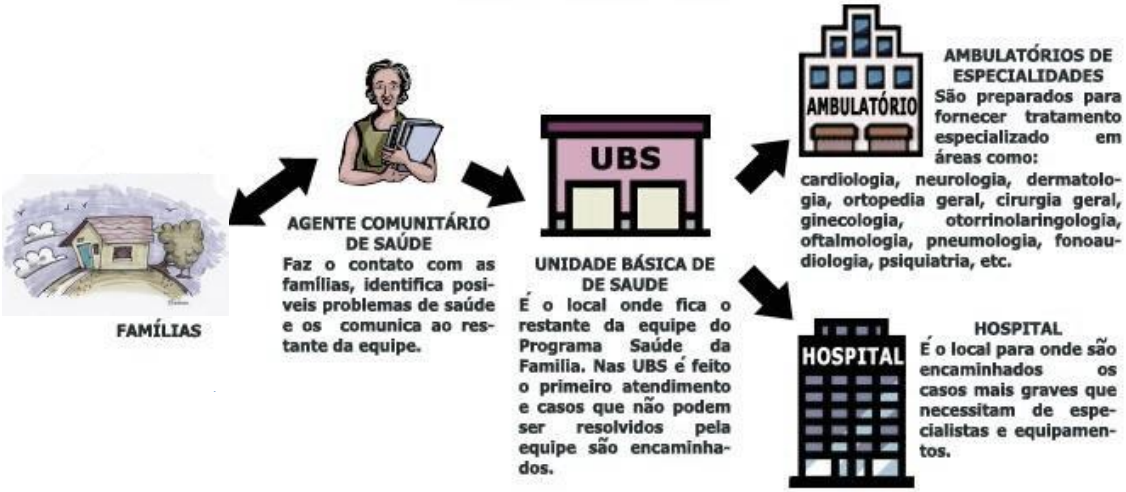
\includegraphics[width=0.9\linewidth]{images/funcionamento-sus.png}
            \fdireta{SECRETARIAMG}
        \end{figure}
    
    Ainda na UBS, caso o paciente necessite de um atendimento emergencial, a \sigla{UPA}{\textit{Unidade de Pronto Atendimento}} é quem o recebe. As UPAs são unidades de complexidade intermediária entre  as UBSs e a emergência dos hospitais, portanto, servem para "desafogar" as filas dos hospitais. Segundo o Ministério da Saúde, 97\% dos casos que chegam as UPAs são solucionados \cite{BRASIL2012}. Os pacientes que procuram as UPAs são avaliados de acordo com a classificação de risco, ou seja, os casos mais graves terão prioridade.
    
    Pode se entender como atendimento secundário, todo atendimento especializado oferecido por hospitais e clínicas. Nesse nível de atendimento,  espera-se que os profissionais estejam preparados para realizar procedimentos de média complexidade, conduzindo o tratamento de quadros que comprometem o bem-estar e a qualidade de vida dos pacientes de forma aguda ou crônica.
    
    O atendimento terciário é o ultimo nível de atenção em saúde no Brasil, por tanto, o mais complexo. É nesse nível que são realizadas cirurgias e exames mais invasivos, que exigem a mais avançada tecnologia em saúde. Ou seja, o nível terciário visa à garantia do suporte mínimo necessário para preservar a vida dos pacientes nos casos em que a atenção no nível secundário não foi suficiente para isso.

     \subsection{Filas de espera}
    
    O caminho que um paciente percorre até o efetivo atendimento pode ser longo e muitas vezes acaba precisando retornar ao início do fluxo de atendimento. O trabalho de \citeonline{SOUZA2014}, avaliou as condições de acesso integral dos usuários a partir do caminho percorrido desde a atenção básica até a especializada na rede assistencial de Recife - PE. O fluxograma do caminho percorrido pelos pacientes é exibido na Figura 2:
    
     \begin{figure}[htbp]
        	\centering
            \caption{Fluxograma descritor do acesso do usuário da atenção primária à atenção especializada.}
            \label{fig:images/fluxograma-trajetoria-usf-pe}
            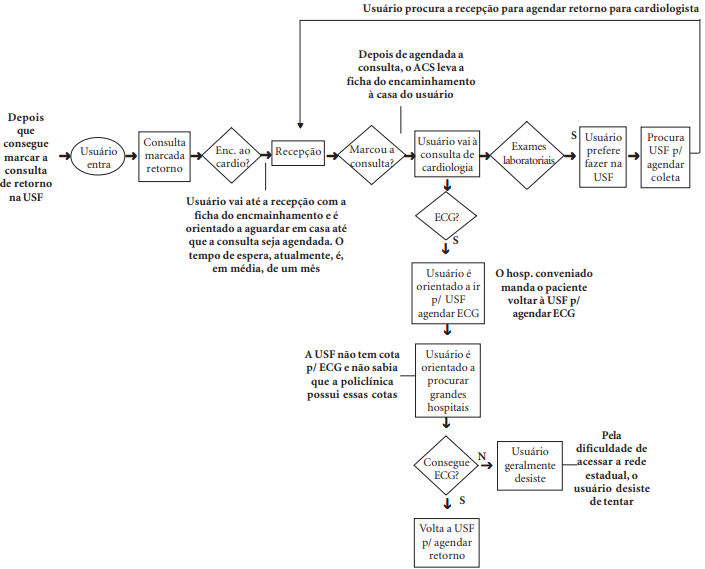
\includegraphics[width=0.8\linewidth]{images/fluxograma-trajetoria-usf-pe}
            \fdireta{SOUZA2014}
        \end{figure}
        
    Quando um médico de família encaminha um usuário ao especialista, esse procura a recepção da USF para entregar a sua ficha de encaminhamento ao profissional responsável pela marcação das consultas que, por sua vez, faz o contato telefônico com a Central de Regulação do Recife para o agendamento.
    
    A demora no agendamento das consultas especializadas é uma das barreiras de acesso para o atendimento integral da população. No estudo, ainda é citado que a inexistência de critérios definidos para a escolha do serviço de referência, no qual os usuários serão agendados, é outro aspecto desordenador do acesso. Essa definição cabe ao pessoal administrativo, ou os ‘marcadores das consultas’. Outro aspecto que chama a atenção, como elemento desordenador, é o fato de o agendamento das consultas ser realizado, predominantemente, pela ordem de chegada das fichas de encaminhamento na recepção. Com exceção dos casos em que o próprio médico sinaliza a ‘urgência’ ou ‘prioridade’ dos pacientes, é o responsável pela marcação das consultas que tenta priorizar
    quem deverá ter acesso e agendamento prioritário. Esse aspecto demonstra que a análise de risco clínico não se coloca como atividade consolidada no processo de trabalho das equipes de saúde da família \cite{SOUZA2014}.
    
    Um outro problema abordado na literatura quando se trata de atendimento especializado, é a questão do absenteísmo. No trabalho de \citeonline{URSULA2018} é realizada uma análise do impacto da fila de espera no absenteísmo de exames e consultas. O estudo revela que as maiores
    probabilidades de ocorrência de absenteísmo são obtidas, de modo geral, em
    procedimentos que ultrapassam os 60 dias de espera. O trabalho afirma que a redução do tempo de espera para menos de 60 dias possibilitou a diminuição significativa do absenteísmo, o que repercute na diminuição do agravamento de doenças e nos custos ao sistema de saúde. 
    
    A fila de espera não é um entrave apenas no SUS, é um problema em cerca da metade dos países da \sigla{OECD}{\textit{Organisation for Economic Co-operation and Development}}  \cite{SICILIANI2004}. Recursos financeiros escassos, quantidade de vagas, gestão e estrutura são também presentes em outros países, como o \sigla{SNS}{\textit{Sistema Nacional de Saúde espanhol}}. No trabalho de \citeonline{CONILL2011}, para o enfrentamento dessas barreiras no acesso ao sistema de saúde, foram realizadas iniciativas que proporcionassem a continuidade assistencial. Foi adotada a medida de circuitos preferenciais. Essa estratégia serve para encaminhar da atenção primária com preferência os usuários com suspeitas de alguma etiologia específica.
    
    Uma parceria entre o Fórum Espanhol de Pacientes em conjunto com a Universidade de Harvard (EUA) desenvolveu uma pesquisa com 3.010 cidadãos para avaliar a confiança dos espanhóis no sistema nacional de saúde. Entre outros aspectos, esse trabalho revelou que, sem distinção de classe social, área geográfica ou densidade demográfica, as listas de espera são o principal problema dos serviços de saúde espanhóis para 78\% dos entrevistados \cite{LOPEZ2007}.
    
    Vale salientar que as filas de espera do atendimento básico para o especializado, não são as únicas onde o paciente encontra problemas, filas como de urgências e cirurgias também são dificuldades reais no SUS. O trabalho de \citeonline{KRISHNAMURTI2005} trás uma abordagem das filas de espera para cirurgias otorrinolaringológicas no SUS. O trabalho descreve que o maior afunilamento acontece na obtenção da consulta no ambulatório de otorrinolaringologia, ou seja, no atendimento especializado (seta nº 3, na figura 3).
    
    \begin{figure}[htbp]
        	\centering
            \caption{Fluxograma de atendimento - as setas tracejadas representam os pontos críticos no processo de obtenção do tratamento.}
            \label{fig:images/fluxo-fila-cirurgia-otorrino}
            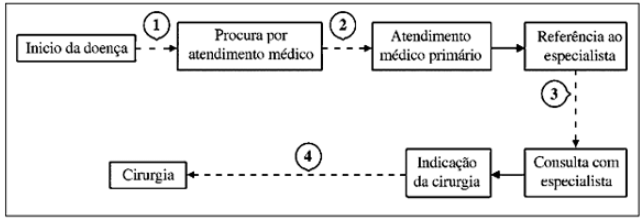
\includegraphics[width=0.9\linewidth]{images/fluxo-fila-cirurgia-otorrino.png}
            \fdireta{KRISHNAMURTI2005}
        \end{figure}
        
    O trabalho ainda discute um tema importante, ao questionar se os indivíduos dessas filas de espera realmente passaram por vias regulares e justas para o atendimento. Muitos que têm a possibilidade, procuram outras formas de obter a consulta, surgem então os pedidos de "consulta extras". São os chamados "PAFs" ou "PAFUNCIOs" tão conhecidos do médico que trabalha em serviço público: "Parente ou Amigo de Funcionário".

    No artigo, o autor relata que ocorre uma pressão não só diretamente sobre os médicos, mas também sobre enfermeiros, auxiliares de enfermagem e demais funcionários. Os funcionários responsáveis pela marcação das consultas também são pressionados, de modo que é preciso atentar para o fato de que mesmo o paciente que parece ter tido a sua consulta marcada por vias regulares pode ter sido beneficiado nessa marcação. Na opnião do autor, já há casos (crimes, citados por ele) de pessoas e funcionários que vendem essas consultas ou mesmo um lugar na fila da triagem do hospital. O médico, sem saber, passa a ser o instrumento de um lucrativo negócio: o do agenciamento da medicina pública \cite{KRISHNAMURTI2005}.
    
    Esses pacientes, independente da gravidade de suas queixas e do seu direito inquestionável ao atendimento, estão na realidade "furando" uma fila virtual de espera. Pode-se chegar a extremos em que o número de pessoas "furando" a fila é tal a ponto de criar uma fila paralela, com fluxo contínuo, enquanto a fila principal e legítima permanece quase parada. Concluindo, o trabalho ainda deixa claro que é necessário o enfrentamento da questão, e que os pacientes devem ser informados sobre sua condição, de preferência por escrito, da indicação cirúrgica, da existência da fila, dos critérios de prioridade nessa fila, da quantidade de pessoas à sua frente e de uma estimativa do tempo até sua cirurgia, deixando-se claro tratar-se apenas de uma estimativa.
    
    % aqui pode-se falar que a falta de critérios de entrada e priorização de atendimento permitem que pacientes possam "furar" a fila, novamente é complicado afirmar que isso ocorre...
    
    %Dilvan- O que o artigo diz? Se ele fala em crime ou furar fila,isso deve ser mantido. Igor,voce nao deve falar nada a mais do que esta no artigo.
    
    %Igor:  conforme relatado no parágrafo, são informações que o autor relata e foram apenas citadas neste trabalho, todas os termos "crimes", "furando fila" foram retirados da forma que é descrita no trabalho
  



    
  